\documentclass{standalone}
\usepackage{tikz}
\usepackage{textcomp}

\begin{document}

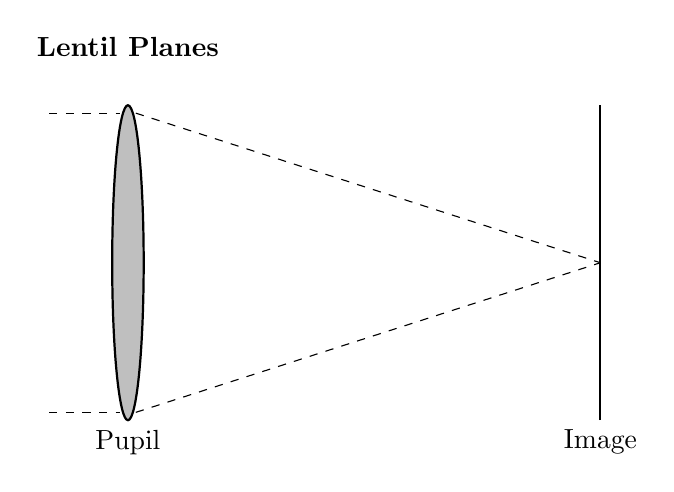
\begin{tikzpicture}

    \node[above] at (0,2.5) {\textbf{Lentil Planes}};
    \draw[thick, fill=lightgray] (0,0) circle [x radius=0.2, y radius=2];
    \node[below] at (0,-2) {Pupil};

        \draw[thick] (6,-2) -- (6,2);
    \node[below] at (6,-2) {Image};

    \draw[dashed](-1,1.9) -- (-0.1,1.9);
    \draw[dashed](0.1,1.9) -- (6,0);
    \draw[dashed](-1,-1.9) -- (-0.1,-1.9);
    \draw[dashed](0.1,-1.9) -- (6,0);

\end{tikzpicture}
\end{document}
